
% spellcheck:
% mikes: (not found)

\chapter{Finding Clusters}{}{}
\label{ch:clustering}

\index{data analysis!clustering|(}
\index{clustering|(}
  
\Fint{The term \emph{clustering} refers to the process of finding groups of
points within a data set that are in} some way ``lumped together.'' It
is also called \emph{unsupervised learning}---unsupervised \index{unsupervised learning} because we
don't know ahead of time where the clusters are located or what they
look like. (This is in contrast to \emph{supervised learning} or
\emph{classification}, where we attempt to assign data points to
preexisting classes; see Chapter \ref{ch:prediction}.)

I regard clustering as an \emph{exploratory} method: a
computer-assisted (or even computationally driven) approach to
discovering structure in a data set. As an exploratory technique, it
usually needs to be followed by a confirmatory analysis that validates
the findings and makes them more precise.

Clustering is a lot of fun. It is a rich topic with a wide variety of
different problems, as we will see in the next section, where we
discuss the different \emph{kinds} of cluster one may encounter. The
topic also has a lot of intuitive appeal, and most clustering methods
are rather straightforward. This allows for all sorts of ad hoc
modifications and enhancements to accommodate the specific problem one
is working on.

% ============================================================
\section{What Constitutes a Cluster?}

\index{clustering!about|(} 

Clustering is not a very rigorous field: there are precious few
established results, rigorous theorems, or algorithmic guarantees. In
fact, the whole notion of a ``cluster'' is not particularly well
defined.  Descriptions such as ``groups of points that are similar''
or ``close to each other'' are insufficient, because clusters must
also be \emph{well separated} from each other. Look at Figure
\ref{fig:uniform}: some points are certainly closer to
each other than to other points, yet there\vadjust{\pagebreak} are no discernible clusters.
(In fact, it is an interesting exercise to define what constitutes the
\emph{absence} of clusters.) This leads to one possible definition of
clusters: \emph{contiguous regions of high data point density
  separated by regions of lower point density}. Although not
particularly rigorous either, this description does seem to capture
the essential elements of typical clusters. (For a different point of
view, see the next section.)

\begin{figure}
  \centerline{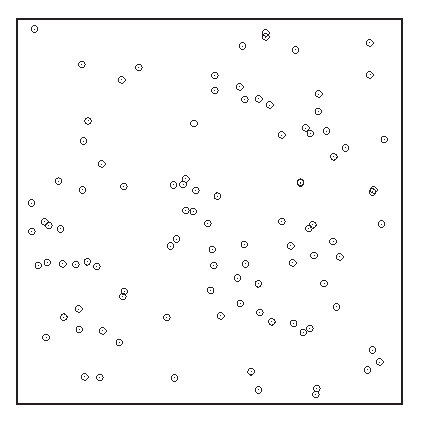
\includegraphics{img/uniform}}
  \caption{A uniform point distribution. Any ``clusters'' that we
    may recognize are entirely spurious.}
  \label{fig:uniform}\vspace*{-6pt}
\end{figure}

The definition just proposed allows for very different kinds of
clusters.  Figures \ref{fig:clouds} and \ref{fig:smiley} show two very
different types. Of course, Figure \ref{fig:clouds} is the ``happy''
case, showing a data set consisting of well-defined and clearly
separated regions of high data point density.  The clusters in Figure
\ref{fig:smiley} are of a different type, one that is more easily
thought of by means of nearest-neighbor (graph) relationships than by
point density.  Yet in this case as well, there are higher density
regions separated by lower density regions---although we might want to
exploit the nearest-neighbor relationship instead of the higher
density when developing with a practical algorithm for this case.

\begin{figure}
  \centerline{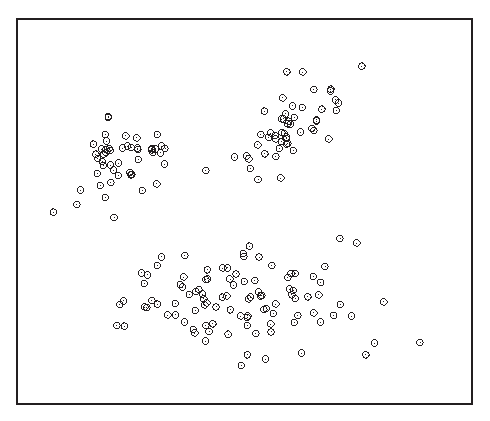
\includegraphics{img/clouds}}
  \caption{The ``happy'' case: three well-separated, globular clusters.}
  \label{fig:clouds}
\end{figure}


\begin{figure}
  \centerline{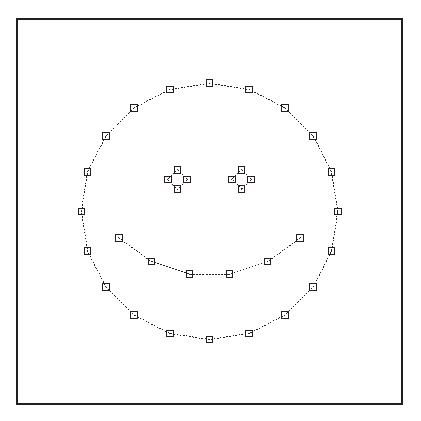
\includegraphics{img/smiley}}
  \caption{Examples of non-globular clusters in a smiley face. Some of
    the clusters are \emph{nested}, meaning that they are entirely
    contained within other clusters.}
  \label{fig:smiley}\vspace*{-6pt}
\end{figure}

Clustering is not limited to points in space. Figures
\ref{fig:stringscluster} and \ref{fig:timeseriescluster} show two
rather different cases for which it nevertheless makes sense to speak
of clusters. Figure \ref{fig:stringscluster} shows a bunch of street
addresses.  No two of them are exactly the same, but if we look
closely, we will easily recognize that all of them can be grouped into
just a few neighborhoods. Figure \ref{fig:timeseriescluster} shows a
bunch of different time series: again, some of them are more alike
than others.  The challenge in both of these examples is finding
a way to express the ``similarity'' among these nonnumeric,
nongeometric objects!


Finally, we should keep in mind that clusters may have complicated
\emph{shapes}. Figure \ref{fig:bananas} shows two very well-behaved
clusters as distinct regions of high point density. However,
complicated and intertwined shapes of the regions will challenge many
commonly used clustering algorithms.

A bit of terminology can help to distinguish different cluster shapes.
If the line connecting any two points lies entirely within the cluster
itself (as in Figure \ref{fig:clouds}), then the cluster is
\emph{convex}. \index{convex clusters} This is the easiest shape to handle.  A cluster is
convex only if the connecting line between two points lies entirely
within the cluster for \emph{all} pairs of points.  Sometimes this is
not the case, but we can still find at least one point (the
\emph{center}) such that the connecting line from the center to any
other point\vadjust{\pagebreak} lies entirely within the cluster: such a cluster is called
\emph{star convex}. \index{star convex clusters} Notice that the clusters in Figure
\ref{fig:bananas} are neither convex nor star convex. Sometimes one
cluster is entirely surrounded by another cluster without actually
being part of it: in this case we speak of a \emph{nested} cluster. \index{nested clusters} 
Nested clusters can be particularly challenging (see Figure
\ref{fig:smiley}).


\begin{figure}
  \centerline{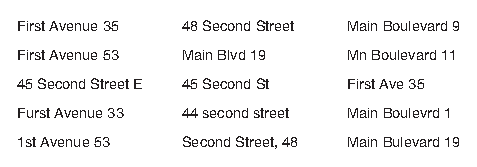
\includegraphics{img/strings}}
  \caption{Clustering strings. Although none of these strings are identical, 
we can make out several groups of strings that are similar to each
other.}
  \label{fig:stringscluster}
\end{figure}

\begin{figure}
  \centerline{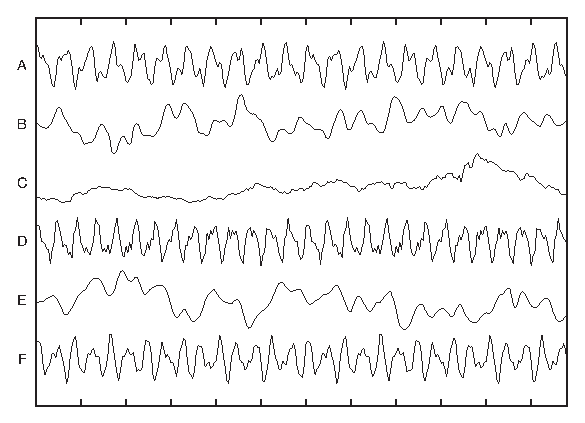
\includegraphics{img/timeseriescluster}}
  \caption{Six time series. We can recognize groups of time series that
    seem more similar to each other than to others.}
  \label{fig:timeseriescluster}\vspace*{-6pt}
\end{figure}


\subsection{A Different Point of View}

In the absence of a precise (mathematical) definition, a cluster can
be whatever we consider as one. That is important because our minds
have a different, alternative way of grouping (``clustering'')
objects: not by proximity or density but rather by the way objects fit
into a larger structure. Figures \ref{fig:crossedclouds} and
\ref{fig:tee} show two examples.


\begin{figure}
  \centerline{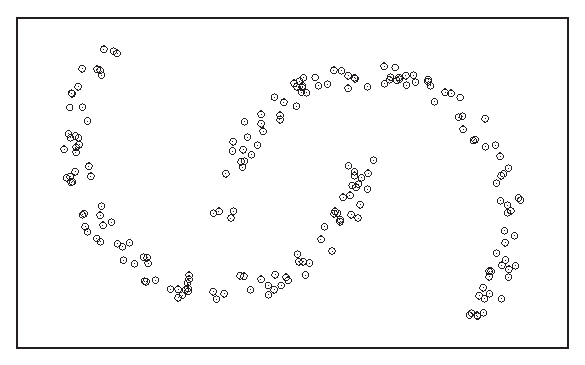
\includegraphics{img/bananas}}
  \caption{Two clusters that are well separated but not globular.
    Some algorithms (\eg, the $k$-means algorithm) will not be able to
    handle such clusters.}
  \label{fig:bananas}
\end{figure}

\begin{figure}
  \centerline{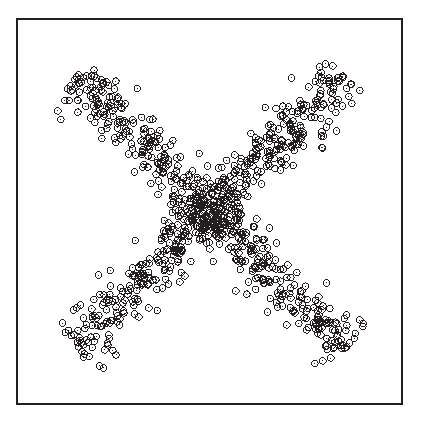
\includegraphics{img/crossedclouds}}
  \caption{An impossible situation for most clustering algorithms:
    although we believe to recognize two crossed clusters, no strictly
    local algorithm will be able to separate them.}
  \label{fig:crossedclouds}
\end{figure}


Intuitively, we have no problem grouping the points in Figure
\ref{fig:crossedclouds} into two overlapping clusters. Yet, the
density-based definition of a cluster we proposed earlier will not
support such a conclusion.  Similar considerations apply to the set of
points in Figure \ref{fig:tee}. The distance between any two adjacent 
points\vadjust{\pagebreak} is the same, but we perceive the larger structures of the
vertical and horizontal arrangements and assign points to clusters
based on them.


\begin{figure}
  \centerline{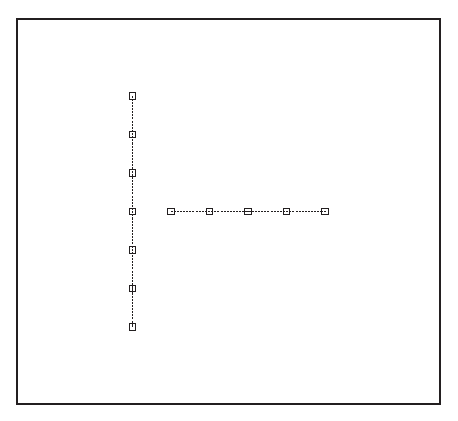
\includegraphics{img/tee}}
  \caption{The two clusters are distinguished not by a local property
    between pairs of points but rather by a global property of the
    entire cluster.}
  \label{fig:tee}
\end{figure}

This notion of a cluster does not hinge on the similarity or proximity
of any pair of points to each other but instead on the similarity
between a point and a property of the \emph{entire cluster}. For any
algorithm that considers a single point (or a single pair of points)
at a time, this leads to a problem: to determine cluster membership,
we need the property of the whole cluster; but to determine the
properties of the cluster, we must first assign points to clusters.

To handle such situations, we would need to perform some kind of
global structure analysis---a task our minds are incredibly good at
(which is why we tend to think of clusters this way) but that we have
a hard time teaching computers to do.  For problems in two dimensions,
\emph{digital image processing} has developed methods to recognize and
extract certain features (such as edge detection). But general
clustering methods, such as those described in the rest of this
chapter, deal only with local properties and therefore can't handle
problems such as those in Figures \ref{fig:crossedclouds} and
\ref{fig:tee}.

\index{clustering!about|)}


% ============================================================
\section{Distance and Similarity Measures}

\index{clustering!distance and similarity measures|(}
\index{distance measures, clustering|(}
\index{similarity measures, clustering|(}   

Given how strongly our intuition about clustering is shaped by
geometric problems such as those in Figures \ref{fig:clouds} and
\ref{fig:smiley}, it is an interesting and perhaps surprising
observation that clustering does not actually require data points to
be embedded into a geometric space: all that is required is a
\emph{distance} or (equivalently) a \emph{similarity measure} for any
\emph{pair of points}. This makes it possible to perform clustering on
a set of strings, such as those in Figure \ref{fig:stringscluster}
that do not map to points in space. However, if the data points have
properties of a vector space (see Appendix \ref{app:data}), then we
can develop more efficient algorithms that exploit these properties.


A \emph{distance} is any function $d(x,y)$ that takes two points and
returns a scalar value that is a measure for how different these
points are: the more different, the larger the distance.  Depending on
the problem domain, it may make more sense to express the same
information in terms of a \emph{similarity} function $s(x,y)$, which
returns a scalar that tells us how similar two points are: the more
different\vadjust{\pagebreak} they are, the smaller the similarity. Any distance can be
transformed into a similarity and vice versa. For example if we know
that our similarity measure $s$ can take on values only in the range
$[0,1]$, then we can form an equivalent distance by setting $d = 1-s$.
In other situations, we might decide to use $d = 1/s$, or $s =
e^{-d}$, and so on; the choice will depend on the problem we are
working on. In what follows, I will express problems in terms of
either distances or similarities, whichever seems more natural. Just
keep in mind that you can always transform between the two.

How we define a distance function is largely up to us, and we can
express different semantics about the data set through the appropriate
choice of distance. For some problems, a particular distance measure
will present itself naturally (if the data points are points in space,
then we will most likely employ the Euclidean distance or a measure
similar to it), but for other problems, we have more freedom to define
our own metric. We will see several examples shortly.

There are certain properties that a distance (or similarity) function
should have. Mathematicians have developed a set of properties that a
function must possess to be considered a metric (or distance) in a
mathematical sense. These properties can provide valuable guidance,
but don't take them too seriously: for our purposes, different
properties might be more important. The four axioms of a mathematical
metric are:
\begin{align*}
d(x,y) & \ge 0 \\
d(x,y) & = 0 \quad \text{if and only if $x=y$} \\
d(x,y) & = d(y,x) \\
d(x,y) + d(y,z) & \ge d(x,z)
\end{align*}

The first two axioms state that a distance is always positive and that
it is null only if the two points are equal. The third property
(``symmetry'') \index{symmetry!clustering} states that the distance between $x$ and $y$ is the
same as the distance between $y$ and $x$---no matter which way we
consider the pair. The final property is the so-called triangle
inequality, which states that to get from $x$ to $z$, it is never
shorter to take a detour through a third point $y$ instead of going
directly (see Figure \ref{fig:triangleeq}).

\begin{figure}
  \centerline{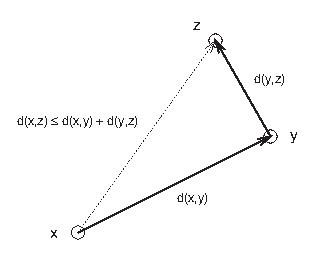
\includegraphics{img/triangleeq}}
  \caption{The triangle inequality: the direct path from $x$ to $z$ is
    always shorter than any path that goes through an intermediate
    point $y$.}
  \label{fig:triangleeq}
\end{figure}

This all seems rather uncontroversial, but these conditions are not
necessarily fulfilled in practice. A funny example for an asymmetric
distance occurs if you ask everyone in a group of people how much they
like every other member of the group and then use the responses to
construct a distance measure: it is not at all guaranteed that the
feelings of person A for person B are requited by B. (Using the same
example, it is also possible to construct scenarios that violate the
triangle inequality.) For technical reasons, the symmetry property is
usually highly desirable. You can always construct a symmetric
distance function from an asymmetric one:
%
\[
d_S(x,y) = \frac{ d(x,y) + d(y,x) }{2} 
\]
%
is always symmetric.

One property of great practical importance but not included among the
distance axioms is \emph{smoothness}. \index{smoothness, clustering} For example, we could define a
rather simple-minded distance function that is $0$ if and only if both
points are equal to each other and that is $1$ if the two points are
not equal:
%
\[
d(x,y) = 
\begin{cases}
  0 & \text{if $x=y$} \\
  1 & \text{otherwise}
\end{cases}
\]
%
You can convince yourself that this distance fulfills all four of the
distance axioms. However, this is not a very informative distance
measure, because it gives us no information about \emph{how} different
two nonidentical points are! Most clustering algorithms require this
information. A certain kind of tree-based algorithm, for example,
works by successively considering the pairs of points with the
smallest distance between them. When using this binary distance, the
algorithm will make only limited progress before having exhausted
all information available to it.

The practical upshot of this discussion is that a good distance
function for clustering should change smoothly as its inputs become
more or less similar. (For classification tasks, a binary one as in
the example just discussed might be fine.)

\subsection{Common Distance and Similarity Measures}

Depending on the data set and the purpose of our analysis, there are
different distance and similarity measures available.

First, let's clarify some terminology. We are looking for ways to
measure the distance between any two data points. Very often, we will
find that a point has a number of \emph{dimensions} or
\emph{features}. (The first usage is more common for numerical data,
the latter for categorical data.) In other words, each point is a
collection of individual values: $x = \braces{x_1, x_2, \dots, x_d}$,
where $d$ is the number of dimensions (or features).  For example, the
data point $\braces{0, 1}$ has two dimensions and describes a point in
space; whereas the tuple\break \texttt{[ 'male', 'retired', 'Florida' ]},
which describes a person, has three features.

For any given data set containing $n$ elements, we can form $n^2$
pairs of points. The set of all distances for all possible pairs of
points can be arranged in a quadratic table known as the
\emph{distance matrix}. \index{distance matrices} The distance matrix embodies all information
about the mutual relationships between all points in the data set. If
the distance function is symmetric, as is usually the case, then the
matrix is also symmetric. Furthermore, the entries along the main
diagonal typically are all $0$, since $d(x,x) = 0$ for most
well-behaved distance functions.

\subsubsection{Numerical data}

\index{numerical data!clustering}
 
If the data is numerical and also``mixable'' or vector-like (in the
sense of Appendix \ref{app:data}), then the data points bear a strong
resemblance to points in space; hence we can use a metric such as the
familiar \emph{Euclidean distance}. \index{Euclidean distance} The Euclidean distance is the most
commonly used from a large family of related distance measures, which
also contains the so-called \emph{Manhattan} \index{Manhattan distance} (or \emph{taxicab})
\emph{distance} \index{taxicab distance} and the \emph{maximum} \index{maximum distance} (or \emph{supremum})
\emph{distance}. \index{supremum distance} All of these are in fact special cases of a more
general \emph{Minkowski} \index{Minkowski distance} or \emph{$p$-distance}.\index{p-distance@$p$-distance}\footnote{The
  Minkowski \emph{distance} defined here should not be confused with
  the Minkowski \emph{metric}, which defines the metric of the
  four-dimensional space-time in special relativity.}  Table
\ref{tbl:distancemeasures} shows some examples. (The Manhattan
distance is so named because it measures distances the way a New York
taxicab moves: at right angles, along the city blocks. The Euclidean
distance measures distances ``as the crow flies.'' Finally, it is an
amusing exercise to show that the maximum distance corresponds to the
Minkowski $p$-distance as $p \to \infty$.)

\begin{table}
\newlength{\clusterlen}
\def\a{\hphantom{0}}
\def\vrl{\smash{\vrule height135pt  width.25pt depth5pt}}
\tbl{Commonly used distance and similarity measures for numeric
data\label{tbl:distancemeasures}}{%
\begin{tabular}{l@{\hskip9pt}c@{\hskip9pt}l}\botrule
\TCH{Name} && \TCH{Definition}  \\\colrule
Manhattan   &&
$d(x, y) = \sum_i^d \abs{x_i - y_i}$ \\[3pt]
Euclidean &&
$d(x, y) = \sqrt{ \sum_i^d \paren{x_i - y_i}^2 }$ \\
Maximum && 
$d(x, y) = \max_i \abs{x_i - y_i}$ \\
Minkowski &&
$d(x, y) = \paren{ \sum_i^d \abs{x_i - y_i}^p }^{1/p}$ \\ \colrule
Dot product & &
$x \cdot y = 
\frac{\sum_i^d x_i y_i}{ \sqrt{\sum_i^d x_i^2} \sqrt{\sum_i^d y_i^2} }$ \\[12pt]
\settowidth{\clusterlen}{Correlation}%
\parbox{\clusterlen}{Correlation coefficient} & &
$\operatorname{corr}(x,y) = 
\frac{\sum_i^d (x_i - \bar{x}) (y_i - \bar{y})}{ 
  \sqrt{\sum_i^d (x_i-\bar{x})^2} \sqrt{\sum_i^d (y_i-\bar{y})^2} }$ \\[12pt]
&\vrl&
$\bar{x} = \frac{1}{d} \sum_i^d x_i \quad  \quad
\bar{y} = \frac{1}{d} \sum_i^d y_i$ \\ 
\botrule
\end{tabular}}
\end{table}


% \begin{table}
% \newlength{\clusterlen}
% \begin{tabular}{|l|l|l|}
% \hline
% Name & General & In 2 dimensions \rule{0mm}{4mm} \\
% \hline
% Manhattan \rule{0mm}{4mm} &
% $d(x, y) = \sum_i^d \abs{x_i - y_i}$ &
% $d(x, y) = \abs{x_1 - y_1} + \abs{x_2 - y_2}$ \\
% Euclidean &
% $d(x, y) = \sqrt{ \sum_i^d \paren{x_i - y_i}^2 }$ &
% $d(x, y) = \sqrt{ \paren{x_1 - y_1}^2 + \paren{x_2 - y_2}^2 }$ \\
% Maximum & 
% $d(x, y) = \max_i \abs{x_i - y_i}$ &
% $d(x, y) = \max( \abs{x_1 - y_1}, \abs{x_2 - y_2} )$ \\
% Minkowski &
% $d(x, y) = \paren{ \sum_i^d \abs{x_i - y_i}^p }^{1/p}$ &
% $d(x, y) = \paren{ \abs{x_1 - y_1}^p + \abs{x_2 - y_2}^p }^{1/p}$ \\
% \hline
% \hline
% Dot product &
% $x \cdot y = 
% \frac{\sum_i^d x_i y_i}{ \sqrt{\sum_i^d x_i^2} \sqrt{\sum_i^d y_i^2} } $ &
% $x \cdot y = 
% \frac{x_1 y_1 + x_2 y_2}{\sqrt{x_1^2 + x_2^2} \sqrt{y_1^2 + y_2^2}}$ \\
% \settowidth{\clusterlen}{Correlation}%
% \parbox{\clusterlen}{Correlation coefficient} &
% $\operatorname{corr}(x,y) = 
% \frac{\sum_i^d (x_i - \bar{x}) (y_i - \bar{y})}{ 
%   \sqrt{\sum_i^d (x_i-\bar{x})^2} \sqrt{\sum_i^d (y_i-\bar{y})^2} }$ &
% $\operatorname{corr}(x,y) = 
% \frac{(x_1 - \bar{x})(y_1 - \bar{y}) + (x_2 - \bar{x})(y_2 - \bar{y})}{
%   \sqrt{x_1^2 + x_2^2} \sqrt{y_1^2 + y_2^2}}$ \\
% &
% $\bar{x} = \frac{1}{d} \sum_i^d x_i \quad ; \quad
% \bar{y} = \frac{1}{d} \sum_i^d y_i$ &
% $\bar{x} = \frac{x_1 + x_2}{2} \quad ; \quad
% \bar{y} = \frac{y_1 + y_2}{2}$ \\
% \hline
% \end{tabular}
% \caption{Commonly used distance measures for numeric data.}
% \label{tbl:distancemeasures}
% \end{table}

All these distance measures have very similar properties, and the
differences between them usually do not matter much. The Euclidean
distance is by far the most commonly used. I list the others here
mostly to give you a sense of the kind of leeway that exists in
defining a suitable distance measure---without significantly affecting
the results!

If the data is numeric but \emph{not} mixable (so that it does not
make sense to add a random fraction of one data set to a random
fraction of a different data set), then these distance measures are
not appropriate. Instead, you may want to consider a metric based on
the \emph{correlation} \index{correlations, clustering} between two data points.

Correlation-based measures are measures of \emph{similarity}: they are
large when objects are similar and small when the objects are
dissimilar. There are two related measures: the \emph{dot product} \index{dot product} and
the \emph{correlation coefficient}, \index{correlation coefficient!clustering} which are also defined in Table
\ref{tbl:distancemeasures}. The only difference is that when
calculating the correlation coefficient, we first center both data
points by subtracting their respective means.

% Don't mention Spearman, Kendall

In both measures, we multiply entries for the same ``dimension'' and
sum the results; then we divide by the correlation of each data point
with itself. Doing so provides a \emph{normalization} and ensures that
the correlation of any point with itself is always $1$. This
normalization step makes correlation-based distance measures suitable
for data sets containing data points with widely different numeric
values.

By construction, the value of a dot product always falls in the
interval $[0,1]$, and the correlation coefficient always falls in the
interval $[-1,1]$. You can therefore transform either one into a
distance measure if need be (\eg, if $d$ is the dot product, then
$1-d$ is a proper distance).

I should point out that the dot product has a geometric meaning. If we
regard the data points as vectors in some suitable space, then the dot
product of two points is the cosine of the angle that the two vectors
make with each other. If they are perfectly aligned (\ie, they fall
onto each other), then the angle is $0$ and the cosine (and the
correlation) is $1$. If they are at right angles to each other, the
cosine is $0$.

\enlargethispage{6pt}

Correlation-based distance measures are suitable whenever numeric data
is not readily mixable---for instance, when evaluating the similarity
of the time series in Figure \ref{fig:timeseriescluster}.

\vspace*{-6pt}      
\subsubsection{Categorical data}

\index{categorical data!clustering} 

If the data is categorical, then we can count the number of features
that do \emph{not} agree in both data points (\ie, the number of
mismatched features); this is the \emph{Hamming distance}. \index{Hamming distance} (We might
want to divide by the total number of features to obtain a number
between $0$ and $1$, which is the \emph{fraction of mismatched
  features}.)

In certain data mining problems, the number of features is large, but
only relatively few of them will be present for each data point.
Moreover, the features may be binary: we care only whether or not they
are present, but their values don't matter.  (As an example, imagine a
patient's health record: each possible medical condition constitutes a
feature, and we want to know whether the patient has ever suffered
from it.)  In such situations, where features are not merely
categorical but binary and sparse (meaning that just a few of the
features are On), we may be more interested in matches between
features that are On than in matches between features
that are Off. This leads us to the \emph{Jaccard coefficient} $s_J$,
\index{Jaccard coefficient and distance} which is the
number\vadjust{\pagebreak} of matches between features that are On for both
points, divided by the number of features that are On in at least one of the
data points. The Jaccard coefficient is a \emph{similarity} measure; the
corresponding distance function is the \emph{Jaccard distance}
$d_J = 1 - s_J$.
\begin{align*}
n_{00} & \quad \text{features that are Off in both points} \\
n_{10} & \quad \text{features that are On in the first point, 
                     and Off in the second point} \\
n_{01} & \quad \text{features that are Off in the first point, 
                     and On in the second point} \\
n_{11} & \quad \text{features that are On in both points} \\
s_J & = \frac{n_{11}}{n_{10} + n_{01} + n_{11}} \\
d_J & = \frac{n_{10} + n_{01}}{n_{10} + n_{01} + n_{11}}
\end{align*}

There are many other measures of similarity or dissimilarity for
categorical data, but the~principles are always the same. You
calculate some fraction of matches, possibly emphasizing one aspect
(\eg, the presence or absence of certain values) more than others.
Feel free to invent your own---as far as I can see, none of these
measures has achieved universal acceptance or is fundamentally better
than any other.

\vspace*{-6pt}
\subsubsection{String data}

\index{string data, clustering}
 
If the data consists of strings, then 
we can use a form of Hamming distance
and count the number of mismatches. If the strings in the data set are
not all of equal length, we can pad the shorter string and count the
number of characters added as mismatches.

If we are dealing with many strings that are rather similar to each
other (distorted through typos, for instance), then we can use a more
detailed measure of the difference between them---namely the
\emph{edit} \index{edit distance} or \emph{Levenshtein distance}. \index{Levenshtein distance} The Levenshtein distance
is the minimum number of single-character operations (insertions,
deletions, and substitutions) required to transform one string into
the other. (A quick Internet search will give many references to the
actual algorithm and available implementations.)

Another approach is to find the length of the \emph{longest common
  subsequence}. \index{longest common subsequence} This metric is often used for gene sequence analysis
in computational biology.

This may be a good place to make a more general point: the best
distance measure to use does not follow automatically from data type;
rather, it depends on the semantics of the data---or, more precisely,
on the semantics that you care about for your current analysis! In
some cases, a simple metric that only calculates the difference in
string length may be perfectly sufficient. In another case, you might
want to use the Hamming distance. If you really care about the details
of otherwise similar strings, the Levenshtein distance is most
appropriate.  You might even want to calculate how often each letter
appears in a string and then base your comparison on
that. It all depends on what the data means and on what
aspect of it you are interested at the moment (which may also change as the
analysis progresses). Similar considerations apply everywhere---there are no
``cookbook'' rules.
      
\subsubsection{Special-purpose metrics}

A more abstract measure for the similarity of two points is based on
the number of neighbors that the two points have in common; this
metric is known as the \emph{shared nearest neighbor} (SNN)
similarity. \index{SNN (shared nearest neighbor) similarity} To calculate the SNN for two points $x$ and $y$, you find
the $k$ nearest neighbors (using any suitable distance function) for
both $x$ and $y$. The number of neighbors shared by both points is
their mutual SNN.

The same concept can be extended to cases in which there is some
property that the two points may have in common. For example, in a
social network we could define the ``closeness'' of two people by the
number of friends they share, by the number of movies they have both
seen, and so on. (This application is equivalent to the Hamming
distance.) Nearest-neighbor-based metrics are particularly suitable
for high-dimensional data, where other distance measures can give
spuriously small results.

% special case: high dim spaces.
% what's the problem? count nbs ... not many there...

Finally, let me remind you that sometimes the solution does not
consist of inventing a new metric. Instead, the trick is to map the
problem to a different space that already has a predefined, suitable
metric.

As an example, consider the problem of measuring the degree of
similarity between different text documents (we here assume that these
documents are long---hundreds or thousands of words). The standard
approach to this problem is to count how often each word appears in
each document. The resulting data structure is referred to as the
\emph{document vector}.\index{document vectors}\index{vectors!document vectors} You can now form a dot product between two
document vectors as a measure of their correspondence.

Technically speaking, we have mapped each document to a point in a
(high-dimensional) vector space. Each distinct word that occurs in any
of the documents spans a new dimension, and the frequency with which
each word appears in a document provides the position of that document
along this axis.  This is very interesting, because we have
transformed highly structured data (text) into numerical, even
vector-like data and can therefore now manipulate it much more easily.
(Of course, the benefit comes at a price: in doing so we have lost all
information about the sequence in which words appeared in the text. It
is a separate consideration whether this is relevant for our purpose.)

One last comment: one can overdo it when defining distance and
similarity measures. Complicated or sophisticated definitions are
usually not necessary as long as you capture the fundamental
semantics. The Hamming distance and the document vector correlation
are two good examples of simplified metrics that intentionally discard
a lot of information yet still turn out to be highly successful in
practice.
\index{clustering!distance and similarity measures|)}
\index{distance measures, clustering|)}
\index{similarity measures, clustering|)}   

\vspace*{-6pt}
% ============================================================
\section{Clustering Methods}

\index{clustering!methods|(} 

In this section, we will discuss several very different clustering
algorithms. As you will see, the basic ideas behind all three
algorithms\vadjust{\pagebreak} are rather simple, and it is straightforward
to come up with perfectly adequate implementations of them yourself. These
algorithms are also important as starting points for more
sophisticated clustering routines, which usually augment them with
various heuristics or combine ideas from different algorithms.

Different algorithms are suitable for different kinds of
problems---depending, for example, on the shape and structure of the
clusters. Some require vector-like data, whereas others require only a
distance function. Different algorithms tend to be misled by different
kinds of pitfalls, and they all have different performance (\ie,
computational complexity) characteristics. It is therefore important
to have a variety of different algorithms at your disposal so that you
can choose the one most appropriate for your problem \emph{and} for
the kind of solution you seek! (Remember: it is pretty much the choice
of algorithm that defines what constitutes a ``cluster'' in the end.)

\vspace*{-6pt}
\subsection{Center Seekers}

\index{k-means algorith@$k$-means algorithm} 

One of the most popular clustering methods is the \emph{$k$-means
  algorithm}. \index{k-means algorith@$k$-means algorithm} The $k$-means algorithm requires the number of expected
clusters $k$ as input. (We will later discuss how to determine this
number.) The $k$-means algorithm is an iterative scheme.  The main
idea is to calculate the position of each cluster's center (or
\emph{centroid}) \index{centroids, clusters} from the positions of the points belonging to the
cluster and then to assign points to their nearest centroid. This
process is repeated until sufficient convergence is achieved. The
basic algorithm can be summarized as follows:

\begin{verbatim}
choose initial positions for the cluster centroids

repeat:
  for each point:
    calculate its distance from each cluster centroid
    assign the point to the nearest cluster

  recalculate the positions of the cluster centroids
\end{verbatim}

The $k$-means algorithm is nondeterministic: a different choice of
starting values may result in a different assignment of
points to clusters. For this reason, it is customary to run the
$k$-means algorithm several times and then compare the results. If you
have previous knowledge of likely positions for the cluster centers,
you can use it to precondition the algorithm. Otherwise, choose random
data points as initial values.

What makes this algorithm efficient is that you don't have to search
the existing data points to find one that would make a good
centroid---instead you are free to \emph{construct} a new centroid
position. This is usually done by calculating the cluster's
center of mass. In two dimensions, we would have:
\begin{gather*}
x_c = \frac{1}{n} \sum_i^n x_i \\
y_c = \frac{1}{n} \sum_i^n y_i
\end{gather*}\vspace*{-6pt}\pagebreak

where each sum is over all points in the cluster. (Generalizations to
higher dimensions are straightforward.)  You can only do this for
vector-like data, however, because only such data allows us to form
arbitrary ``mixtures'' in this way.

For strictly categorical data (such as the strings in Figure
\ref{fig:stringscluster}), the $k$-means algorithm cannot be used
(because it is not possible to ``mix'' different points to construct a
new centroid). Instead, we have to use the \emph{$k$-medoids}
algorithm. \index{k-medoids algorithm@$k$-medoids algorithm}  The $k$-medoids algorithm works in the same way as the
$k$-means algorithm except that, instead of calculating the new
centroid, we search through all points in the cluster to find the data
point (the \emph{medoid}) that has the smallest average distance to
all other points in the cluster.

The $k$-means algorithm is surprisingly modest in its resource
consumption. On each iteration, the algorithm evaluates the distance
function once for each cluster and each point; hence the computational
complexity per iteration is $\mathcal{O}(k \cdot n)$, where $k$ is the
number of clusters and $n$ is the number of points in the data set.
This is remarkable because it means that the algorithm is
\emph{linear} in the number of points. The number of iterations is
usually pretty small: 10--50 iterations are typical. The $k$-medoids
algorithm is more costly because the search to find the medoid of each
cluster is an $\mathcal{O}(n^2)$ process. For very large data sets
this might be prohibitive, but you can try running the $k$-medoids
algorithm on random \emph{samples} of all data points. The results
from these runs can then be used as starting points for a run using
the full data set.

Despite its cheap-and-cheerful appearance, the $k$-means algorithm
works surprisingly well. It is pretty fast and relatively robust.
Convergence is usually quick. Because the algorithm is simple and
highly intuitive, it is easy to augment or extend it---for example,
to incorporate points with different weights. You might also want to
experiment with different ways to calculate the centroid, possibly
using the median position rather than the mean, and so on. 

That being said, the $k$-means algorithm can fail---annoyingly in
situations that exhibit especially strong clustering!  Because of its
iterative nature, the algorithm works best in situations that involve
gradual density changes. If your data sets consists of very dense and
widely separated clusters, then the $k$-means algorithm can get
``stuck'' if initially two centroids are assigned to the same cluster:
moving one centroid to a different cluster would require a large move,
which is not likely to be found by the mostly local steps taken by the
$k$-means algorithm.

Among variants, a particularly important one is \emph{fuzzy
  clustering}. \index{fuzzy clustering} In fuzzy clustering, we don't assign each point to a
single cluster; instead, for each point and each cluster, we determine
the probability that the point belongs to that cluster. Each point
therefore acquires a set of $k$ probabilities or weights (one for each
cluster; the probabilities must sum to $1$ for each point). We then
use these probabilities as weights when calculating the centroid
positions.  The probabilities also make it possible to declare certain
points as ``noise'' (having low probability of\vadjust{\pagebreak} belonging to \emph{any}
cluster) and thus can help with data sets that contain unclustered
``noise'' points and with ambiguous situations such as the one shown
in Figure \ref{fig:crossedclouds}.

To summarize: 

\begin{itemize}
\item The $k$-means algorithms and its variants work best for globular
  (at least star-convex) clusters. The results will be meaningless for
  clusters with complicated shapes and for nested clusters (Figures
  \ref{fig:bananas} and \ref{fig:smiley}, respectively).
\item The expected number of clusters is required as an input. If this
  number is not known, it will be necessary to repeat the algorithm 
  with different values and compare the results.
\item The algorithm is iterative and nondeterministic; the specific
  outcome may depend on the choice of starting values.
\item The $k$-means algorithm requires vector data; use the
  $k$-medoids algorithm for categorical data.
\item The algorithm can be misled if there are clusters of highly
  different size or different density.
\item The $k$-means algorithm is linear in the number of data points;
  the $k$-medoids algorithm is quadratic in the number of points.\vspace*{-3pt}
\end{itemize}

\subsection{Tree Builders}

\index{agglomerative hierarchical clustering} 

Another way to find clusters is by successively combining clusters
that are ``close'' to each other into a larger cluster until only a
single cluster remains. This approach is known as \emph{agglomerative
  hierarchical clustering}, \index{agglomerative hierarchical clustering} and it leads to a treelike hierarchy of
clusters. Clusters that are close to each other are joined early (near
the leaves of the tree) and more distant clusters are joined late (near
the root of the tree). (One can also go in the opposite direction,
continually splitting the set of points into smaller and smaller
clusters. When applied to classification problems, this leads to a
\emph{decision tree}---see Chapter \ref{ch:prediction}.)

The basic algorithm proceeds exactly as just outlined:

\begin{enumerate}
\item Examine all pairs of clusters.
\item Combine the two clusters that are closest to each other into a
  single cluster.
\item Repeat.
\end{enumerate}

What do we mean by the distance \index{distance measures, clustering} between \emph{clusters}? The distance
measures that we have defined are valid only between points! To apply
them, we need to select (or construct) a single ``representative''
point from each cluster. Depending on this choice, hierarchical
clustering will lead to different results. The most important
alternatives are as follows.

\begin{unnumlist}
\subparagraph{Minimum or single link}
\item
We define the distance between two
  clusters as the distance between the two points (one from each
  cluster)\vadjust{\pagebreak} that are \emph{closest} to each other.  This
choice leads
  to extended, thinly connected clusters. Because of this, this
  approach can handle clusters of complicated shapes, such as those in
  Figure \ref{fig:bananas}, but it can be sensitive to noise points.

\subparagraph{Maximum or complete link}
\item
The distance between two clusters is
  defined as the distance between the two points (one from each cluster)
  that are \emph{farthest away} from each other. With this choice, two
  clusters are not joined until all points within each cluster are 
  connected to each other---favoring compact, globular clusters.

\subparagraph{Average}
\item
In this case, we form the average over the distances
  between all pairs of points (one from each cluster).  This choice
  has characteristics of both the single- and complete-link
  approaches.

\subparagraph{Centroid}\index{centroids, clusters}
\item
For each cluster, we
calculate the position of a 
  centroid (as in $k$-means clustering) and define the distance between
  clusters as the distance between centroids.

\subparagraph{Ward's method}
\item
Ward's method \index{Ward's method} measures
the distance between two
  clusters in terms of the decrease in coherence that occurs when the
  two clusters are combined: if we combine clusters that are closer
  together, the resulting cluster should be more coherent than if we
  combine clusters that are farther apart. We can measure coherence as
  the average distance of all points in the cluster from a centroid,
  or as their average distance from each other. (We'll come back to
  cohesion and other cluster properties later.)
\end{unnumlist}

The result of hierarchical clustering is not actually a set of
clusters.  Instead, we obtain a treelike structure that contains the
individual data points at the leaf nodes. This structure can be
represented graphically in a \emph{dendrogram} \index{dendrograms} (see Figure
\ref{fig:dendrogram}). To extract actual clusters from it, we need to
walk the tree, evaluate the cluster properties for each subtree, and
then cut the tree to obtain clusters.

\begin{figure}
  \centerline{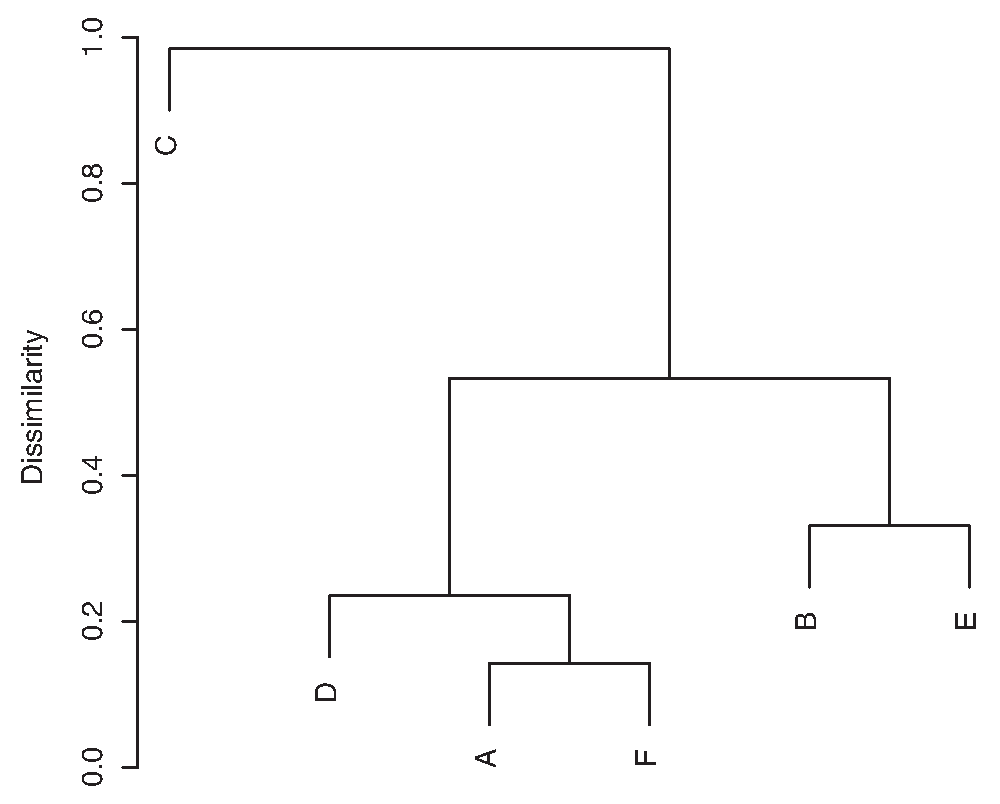
\includegraphics[width=0.8\textwidth]{img/dendrogram}}
  \caption{A typical dendrogram for data like the data in Figure
    \ref{fig:timeseriescluster}. Individual data points are at the
    leaf nodes. The vertical distance between the tree nodes
    represents the dissimilarity between the nodes.}
  \label{fig:dendrogram}
\end{figure}

Tree builders are expensive: we need at least the full distance matrix
for all pairs of points (requiring $\mathcal{O}(n^2)$ operations to
evaluate). Building the complete tree takes $\mathcal{O}(n)$
iterations: there are $n$ clusters (initially, points) to start with,
and at each iteration, the number of clusters is reduced by one because
two clusters are combined. For each iteration, we need to search the
distance matrix for the closest pair of clusters---naively
implemented, this is an $\mathcal{O}(n^2)$ operation \index{O@$\mathcal{O}(n^2)$ operations} that leads to a
total complexity of $\mathcal{O}(n^3)$ operations. However, this can
be reduced to $\mathcal{O}(n^2 \log n)$ by using indexed lookup.

One outstanding feature of hierarchical clustering is that it does
more than produce a flat list of clusters; it also shows their
relationships in an explicit way. You need to decide whether this
information is relevant for your needs, but keep in mind that the
choice of measure for the cluster distance (single- or complete-link,
and so on) can have a significant influence on the appearance of the
resulting tree structure.

\subsection{Neighborhood Growers}

\index{neighborhood growers algorithm}
 
A third kind of clustering algorithm could be dubbed ``neighborhood
growers.'' They work by connecting points that are ``sufficiently
close'' to each other to form a cluster and then keep doing so until
all points have been classified. This approach makes the most direct
use of the definition of a cluster as a region of high density, and it
makes no assumptions about the overall \emph{shape} of the cluster.
Therefore, such methods can handle clusters of complicated shapes (as
in Figure \ref{fig:bananas}), interwoven clusters, or even nested
clusters (as in Figure \ref{fig:smiley}). In general,
neighborhood-based clustering algorithms are more of a special-purpose
tool: either for cases that other algorithms don't handle well (such
as the ones just mentioned) or for polishing, in a second pass, the
features of a cluster found by a general-purpose clustering algorithm
such as $k$-means.

The DBSCAN algorithm \index{DBSCAN algorithm} which we will introduce in this section is one
such algorithm, and it demonstrates some typical concepts. It requires
two parameters. One is the \emph{minimum density} that we expect to
prevail inside of a cluster---points that are less densely packed will
not be considered part of any cluster. The other parameter is the
\emph{size of the region} over which we expect this density to be
maintained: it should be larger than the average distance between
neighboring points but smaller than the entire cluster.  The choice of
parameters is rather subtle and clearly requires an appropriate
balance.

In a practical implementation, it is easier to work with two slightly
different parameters: the neighborhood radius $r$ and the minimum
number of points $n$ that we expect to find within the neighborhood of
each point in a cluster. The DBSCAN algorithm distinguishes between
three types of points: noise, edge, and core points. A \emph{noise
  point} is a point which has fewer than $n$ points in its
neighborhood of radius $r$, such a point does not belong to any
cluster. A \emph{core point} of a cluster has more than $n$ neighbors.
An \emph{edge point} is a point that has fewer neighbors than required
for a core point but that is itself the neighbor of a core point.  The
algorithm discards noise points and concentrates on core points.
Whenever it finds a core point, the algorithm assigns a cluster label
to that point and then continues to add all its neighbors, and
\emph{their} neighbors recursively to the cluster, until all points
have been classified.

% \cit not possible in footnote below
This description is simple enough, but actually deriving a concrete
implementation that is both correct and efficient is less than
straightforward.  The pseudo-code in the original paper\footnote{``A
  Density-Based Algorithm for Discovering Clusters in Large Spatial
  Databases with Noise.'' Martin Ester, Hans-Peter Kriegel, J\"org
  Sander, and Xiaowei Xu. Proceedings of 2nd International Conference
  on Knowledge Discovery and Data Mining (KDD-96). 1996.}  appears
needlessly clumsy; on the other hand, I am not convinced that the
streamlined version that can be found (for example) on Wikipedia is
necessarily correct. Finally, the basic algorithm lends itself to
elegant recursive implementations, but keep in mind that the recursion
will not unwind until the current cluster is complete.  This means
that, in the worst case (of a single connected cluster), you will end
up putting the entire data set onto the stack!

As pointed out earlier, the main advantage of the DBSCAN algorithm is
that it handles clusters of complicated shapes and nested clusters
gracefully. However, it does depend sensitively on the appropriate
choice of values for its two control parameters, and it provides
little help in finding them. If a data set contains several clusters
with widely varying densities, then a single set of parameters may not
be sufficient to classify all of the clusters. These problems can be
ameliorated by coupling the DBSCAN algorithm with the $k$-means
algorithm: in a first pass, the $k$-means algorithm is used to
identify candidates for clusters. Moreover, statistics on these
subsets of points (such as range and density) can be used as input to
the DBSCAN algorithm.

The DBSCAN algorithm is dominated by the calculations required to find
the neighboring points. For each point in the data set, all other
points have to be checked; this leads to a complexity of
$\mathcal{O}(n^2)$. In principle, algorithms and data structures exist
to find candidates for neighboring points more efficiently (\eg,
$kd$-trees and global grids), but their implementations are subtle and
carry their own costs (grids can be very memory intensive). Coupling
the DBSCAN algorithm with a more efficient first-pass algorithm (such
as $k$-means) may therefore be a better strategy.

\index{clustering!methods|)} 

% ============================================================
\section{Pre- and Postprocessing}

\index{clustering!pre- and postprocessing|(} 

The core algorithm for grouping data points into clusters is usually
only part (though the most important one) of the whole strategy. Some
data sets may require some cleanup or normalization before they are
suitable for clustering: that's the first topic in this section.

Furthermore, we need to inspect the results of every clustering
algorithm in order to validate and characterize the clusters that have
been found.  We will discuss some concepts and quantities used to
describe clusters and to measure the clustering quality.

Finally, several cluster algorithms require certain input parameters
(such as the number of clusters to find), and we need to confirm that
the values we provided are consistent with the outcome of the
clustering process. That will be our last topic in this section.

\subsection{Scale Normalization}

\index{scale normalization, clustering}
\index{normalization!scale normalization: clustering} 
 
Look at Figures \ref{fig:unscaled} and \ref{fig:scaled}. Wouldn't you
agree that the data set in Figure \ref{fig:unscaled} exhibits two
reasonably clearly defined and well-separated clusters while the data
set in Figure \ref{fig:scaled} does not? Yet both figures show the
\emph{same} data set---only drawn to different scales! In Figure
\ref{fig:scaled}, I used identical units for both the $x$ axis and the
$y$ axis; whereas Figure \ref{fig:unscaled} was drawn to maintain a
suitable aspect ratio for this data set.

This example demonstrates that clustering is not independent of the
units in which the data is measured. In fact, for the data set shown
in Figures \ref{fig:unscaled} and \ref{fig:scaled}, points in two
different clusters may be closer to each other than to other points in
the same cluster! This is clearly a problem.

If, as in this example, your data spans very different ranges along
different dimensions, you need to normalize the data before starting a
clustering algorithm. An easy way to achieve this is to divide the
data, dimension for dimension, by the range of the data along that
dimension.  Alternatively, you might want to divide by the standard
deviation along that dimension. This process is sometimes called
\emph{whitening} \index{whitening} or \emph{prewhitening}, \index{prewhitening}
particularly in signal-theoretic literature.


\begin{figure}
  \centerline{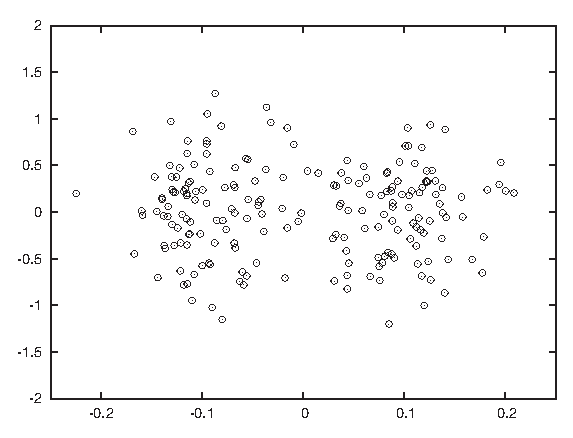
\includegraphics{img/unscaled}}
  \caption{It is easy to argue that there are \emph{two} clusters 
    in this graph. (Compare Figure \ref{fig:scaled}.)}
  \label{fig:unscaled}\vspace*{-6pt}
\end{figure}

% --- XXX : can we refer to PCA and whitening along the PCA axis?

You only need to worry about this problem if you are working with
vector-like data and are using a distance measure like the Euclidean
distance. It does not affect correlation-based similarity measures.
In fact, there is a special variant of the Euclidean distance that
performs the appropriate rescaling for each dimension on the fly: the
\emph{Mahalanobis distance}.

% \soon{Optional: Mahalanobis Distance}
      
\subsection{Cluster Properties and Evaluation}

It is easiest to think about cluster properties in the context of
vector-like data and a straightforward clustering algorithm\vadjust{\pagebreak} such as
$k$-means. The algorithm already gives us the coordinates of the
cluster centroids directly, hence we have the cluster \emph{location}. \index{location, clusters} 
Two additional quantities are the \emph{mass} \index{mass, clusters} of the
cluster (\ie, the number of points in the cluster) and its radius. The
\emph{radius} \index{radius, clusters} is simply the average deviation of
all points from the cluster center---basically the standard deviation, when
using the Euclidean distance:\vspace*{-3pt}
%
\[
r^2 = \sum_i ( x_c - x_i )^2 + ( y_c - y_i )^2\vspace*{-3pt} 
\]
%
in two dimensions (equivalently in higher dimensions). Here $x_c$ and
$y_c$ are the coordinates of the center of the cluster, and the sum
runs over all points $i$ in the cluster. Dividing the mass by the
radius gives us the \emph{density} \index{density, clusters} of the cluster. (These values can
be used to construct input values for the DBSCAN algorithm.)

% something about radius and pre-whitening!
% (could also talk about inertia tensor and diagonalization)

\begin{figure}
  \centerline{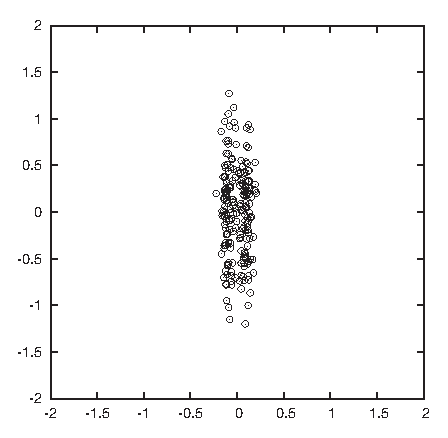
\includegraphics{img/scaled}}
  \caption{It is difficult to recognize two well-separated clusters in this figure. Yet the data is
    the same as in Figure \ref{fig:unscaled} but drawn to a different
    scale! (Compare the horizontal and vertical scales in both
    graphs.)}
  \label{fig:scaled}
\end{figure}     

We can apply the same principles to develop a measure for the overall
quality of the clustering. The key concepts are \emph{cohesion} \index{cohesion, clusters} within
a cluster and \emph{separation} \index{separation, clusters} between clusters. The average distance
for all points within one cluster is a measure of the cohesion, and the
average distance between all points in one cluster from all points in
another cluster is a measure of the separation between the two clusters.
(If we know the centroids of the clusters, we can use the distance
between the centroids as a measure for the separation.)  We can go
further and form the average (weighted by the cluster mass) of the
cohesion for all clusters as a measure for the overall quality.

If a data set can be cleanly grouped into clusters, then we expect the
distance between the clusters to be large compared to the radii of the
clusters.  In other words, we expect the ratio:\vspace*{-3pt}
%
\[
\frac{\text{separation}}{\text{cohesion}}\vspace*{-3pt}
\]
%
to be large.

A particular measure based on this concept is the \emph{silhouette
  coefficient} $S$. \index{silhouette coefficient $S$} The silhouette coefficient is defined for
individual points as follows. Let $a_i$ be the average distance (the
cohesion) that point $i$ has from all other points in the cluster to
which it belongs. Evaluate the average distance that point $i$ has
from all points in any cluster to which it does \emph{not} belong, and
let $b_i$ be the smallest such value (\ie, $b_i$ is the separation from
the ``closest'' other cluster). Then the silhouette coefficient of
point $i$ is defined as:
%
\[
S_i = \frac{ b_i - a_i }{\max( a_i, b_i )}
\]
%
The numerator is a measure for the ``empty space'' between clusters
(\ie, it measures the amount of distance between clusters
that is not occupied by the original cluster). The denominator is the
greater of the two length scales in the problem---namely the cluster
radius and the distance between clusters.

By construction, the silhouette coefficient ranges from $-1$ to $1$.
Negative values indicate that the cluster radius is \emph{greater}
than the distance between clusters, so that clusters overlap; this
suggests poor clustering. Large values of $S$ suggest good clustering.
We can form the average of the silhouette coefficients for all points
belonging to a single cluster and thereby develop a measure for the
quality of the entire cluster. We can further define the average over
the silhouette coefficients for all individual points as the overall
silhouette coefficient for the entire data set; this would be a
measure for the quality of the clustering result.
      
\begin{figure}
  \centerline{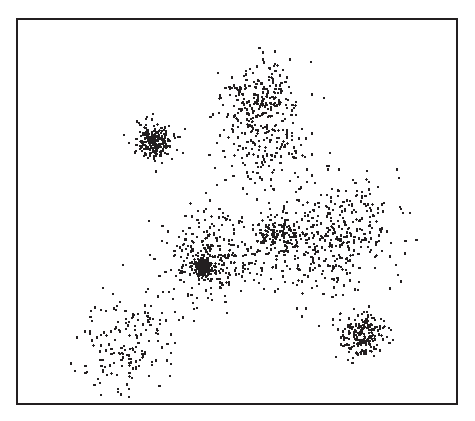
\includegraphics{img/clustershop1}}
  \caption{How many clusters are in this data set?}
  \label{fig:silhouette1}\vspace*{-9pt}
\end{figure}

The overall silhouette coefficient can be useful to determine the number
of clusters present in the data set. If we run the $k$-means\vadjust{\pagebreak} algorithm
several times for different values of the expected number of clusters
and calculate the overall silhouette coefficient each time, then it
should exhibit a peak near the optimal number of clusters.

Let's work through an example to see how the the silhouette
coefficient performs in practice.  Figure \ref{fig:silhouette1} shows
the points of a two-dimensional data set.  This is an interesting data
set because, even though it exhibits clear clustering, it is not at
all obvious how many \emph{distinct} clusters there really are---any
number between six and eight seems plausible.  The total silhouette
coefficient (averaged over all points in the data set) for this data
set (see Figure \ref{fig:silhouette2}) confirms this expectation,
clearly leaning toward the lower end of this range. (It is interesting
to note that the data set was generated, using a random-number
generator, to include \emph{10} distinct clusters, but some of those
clusters are overlapping so strongly that it is not possible to
distinguish them.) This example also serves as a cautionary reminder
that it may not always be so easy to determine what actually
constitutes a cluster!
      
\begin{figure}
  \centerline{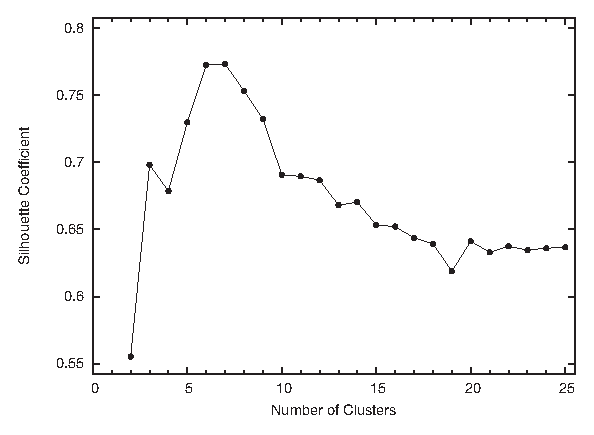
\includegraphics{img/clustershop2}}
  \caption{The silhouette coefficient for the data in Figure
    \ref{fig:silhouette1}. According to this measure, six or seven
    clusters give optimal results for this data set.}
  \label{fig:silhouette2}\vspace*{-6pt}
\end{figure}

Another interesting question concerns distinguishing legitimate
clusters from a random (unclustered) background. Of the algorithms
that we have seen, only the DBSCAN algorithm \index{DBSCAN algorithm} explicitly labels some 
points as background; the $k$-means and the tree-building algorithm
perform what is known as \emph{complete clustering} \index{complete clustering} by assigning every
point to a cluster. We may want to relax this behavior by trimming
those points from each cluster that exceed the average cohesion within
the cluster by some amount.  This is easiest for fuzzy clustering
algorithms, but it can be done for other algorithms as well.
\index{clustering!pre- and postprocessing|)} 

\vspace*{-9pt}
% ============================================================
\section{Other Thoughts}

\index{clustering!issues|(}
  
The three types of clustering algorithms introduced in this chapter
are probably the most~popular and widely\vadjust{\pagebreak} used, but they certainly
don't exhaust the range of possibilities. Here is a brief list of
other ideas that can (and have) been used to develop clustering
algorithms.

\begin{itemize}
\item We can impose a specific \emph{topology}, such as a grid on the
  data points. Each data point will fall into a single grid cell, and
  we can use this information to find cells containing unusually many
  points and so guide clustering.  Cell-based methods will perform
  poorly in many dimensions, because most cells will be empty and have
  few occupied neighbors (the ``curse of dimensionality'').
  
\item Among grid-based approaches, Kohonen maps (which we will discuss
  in Chapter \ref{ch:reduction}) have a lot of intuitive appeal.

\item Some special methods have been suggested to address the
  challenges posed by high-dimensional feature spaces. In
  \emph{subspace clustering}, \index{subspace clustering} for example, clustering is performed on
  only a subset of all available features. These results are then
  successively extended by including features ignored in previous
  iterations.

\item Remember kernel density estimates (KDEs) from Chapter
  \ref{ch:univariate}? \index{KDEs (kernel density estimates)} If the dimensionality is not too high, then we
  can generate a KDE for the data set. The KDE provides a smooth
  approximation to the local point density. We can then identify
  clusters by finding the maxima of this density directly, using
  standard methods from numerical analysis.

\item The QT (``quality threshold'') algorithm \index{QT (``quality threshold'') algorithm} is a center-seeking
  algorithm that does not require the number of clusters as input;
  instead, we have to fix a maximum \emph{radius}. The QT algorithm
  treats \emph{every} point in the cluster as a potential centroid and
  adds neighboring points (in the order of increasing distance from
  the centroid) until the maximum radius is exceeded.  Once\vadjust{\pagebreak} all
  candidate clusters have been completed in this way, the cluster with
  the greatest number of points is removed from the data set, and then
  the process starts again with the remaining points.
      
\item There is a well-known correspondence between graphs and distance
  matrices. Given a set of points, a graph tells us which points are
  directly connected to each other---but so does a distance matrix! \index{distance matrices} 
  We can exploit this equivalence by treating a distance matrix as the
  adjacency matrix of a graph. The distance matrix is pruned (by
  removing connections that are too long) to obtain a sparse graph,
  which can be interpreted as the backbone of a cluster.

\item Finally, \emph{spectral clustering} \index{spectral clustering} uses powerful but abstract
  methods from linear algebra (similar to those used for principal
  component analysis; see Chapter \ref{ch:reduction}) to structure and
  simplify the distance matrix.
\end{itemize}

Obviously, much depends on our prior knowledge about the data set: if
we expect clusters to be simple and convex, then the $k$-means
algorithm suggests itself.  On the other hand, if we have a sense for
the typical radius of the clusters that we expect to find, then QT
clustering would be a more natural approach. If we expect clusters of
complicated shapes or nested clusters, then an algorithm like DBSCAN
will be required.  Of course, it might be difficult to develop this
kind of intuition---especially for problems that have significantly
more than two or three dimensions!

% computational complexity: may be dominated by distance calc in
% high-dim spaces. In that case, medoids might be better than kmeans.
%
% density of cluster only makes sense when using Minkowski distances.
% does not really make sense when using correlation as measure

Besides thinking of different ways to combine points into clusters, we
can also think of different ways to define clusters to begin with. All
methods discussed so far have relied (directly or indirectly) on the
information contained in the distance between any two points. We can
extend this concept and begin to think about \emph{three-point} (or
higher) \emph{distance functions}. For example, it is possible to
determine the \emph{angle} between any three consecutive points and
use this information as the measure of the similarity between points. Such
an approach might help with cases like the one shown in Figure
\ref{fig:tee}. Yet another idea is to measure not the similarity
between \emph{points} but instead the similarity between a point and a
\emph{property of the cluster}. For example, there is a
straightforward generalization of the $k$-means algorithm in which the
centroids are no longer pointlike but are straight lines, representing
the ``axis'' of an elongated cluster. Rather than measuring the
distance for each point from the centroid, this algorithm calculates
the distance from this axis when assigning points to clusters. This
algorithm would be suitable for cases like that shown in Figure
\ref{fig:crossedclouds}. I don't think any of these ideas that try to
generalize beyond pairwise distances have been explored in detail yet.
  
\index{clustering!issues|)}

% ============================================================
\section{A Special Case: Market Basket Analysis}

\index{clustering!market basket analysis example} 
\index{market basket analysis}
\index{association analysis}
  
Which items are frequently bought together? This and similar questions
arise in \emph{market basket analysis} or---more generally---in
\emph{association analysis}. Because association analysis is looking
for items that occur together, it is in some ways related to
clustering. However, the specific nature of the problem is different
enough to require a separate toolset.

The starting point for association analysis is usually a data set
consisting of \emph{transactions}---\break that is, items that have been
purchased together (we will often stay with the market basket metaphor
when illustrating these concepts). Each transaction corresponds to a
single ``data point'' in regular clustering.

For each transaction, we keep track of all items that have occurred
together but typically ignore whether or not any particular item was
purchased multiple times: all attributes are Boolean and indicate only
the presence or absence of a certain item.  Each item spans a new
dimension: if the store sells $N$ different items, then each
transaction can have up to $N$ different (Boolean) attributes,
although each transaction typically contains only a tiny subset of the
entire selection. (Note that we do not necessarily need to know the
dimensionality $N$ ahead of time: if we don't know it, we can infer an
approximation from the number of different items that actually occur
in the data set.)

From this description, you can already see how association analysis
differs from regular clustering: data points in association analysis
are typically very high-dimensional but also very sparse.  It also
differs from clustering (as we have discussed it so far) in that we
are not necessarily interested in grouping entire ``points'' (\ie,
transactions) but would like to identify those dimensions that
frequently occur together.

A group of zero or more items occurring together is known as an
\emph{item set} \index{item sets} (or \emph{itemset}). Each transaction consists of an
item set, but every one of its subsets is also an item set. We can
construct arbitrary item sets from the selection of available items.
For each such item set, its \emph{support count} \index{support count} is the number of
actual transactions that contain the candidate item set as a subset.

Besides simply identifying frequent item sets, we can also try to
derive \emph{association rules}---that is, rules of the form ``if items
A and B are bought, then item C is also likely to be bought.'' Two
measures are important when evaluating the strength of an association
rule: its support $s$ and its confidence $c$. The \emph{support} of a
rule is the fraction of transactions in the entire data set that
contain the combined item set (\ie, the fraction of transactions that
contain all three items A, B, and C). A rule with low support is not
very useful because it is rarely applicable.

The \emph{confidence} \index{confidence, association rules} is a measure for the reliability of an
association rule. It is defined as the number of transactions in which
the rule is \emph{correct}, divided by the number of transactions in
which it is \emph{applicable}. In our example, it would be the number
of times A, B, and C occur together divided by the number of times A
and B occur together.

How do we go about finding frequent item sets (and association rules)?
Rather than performing an open-ended search for the ``best''
association rule, it is customary to set thresholds for the minimum
support (such as 10 percent) and confidence (such as 80 percent)
required of a rule and then to generate all rules that meet these
conditions.

To identify rules, we generate candidate item sets and then evaluate
them against the set of transactions to determine whether they exceed
the required thresholds. However, the naive approach---to create and
evaluate \emph{all} possible item sets of $k$ elements---is not
feasible because of the huge number ($2^k$) of candidate item sets
that could be generated, most of which will \emph{not} be frequent! We
must find a way to generate candidate item sets more efficiently.

The crucial observation is that \emph{an item set can occur
  frequently only if all of its subsets occur frequently}. This
insight is the basis for the so-called \emph{apriori algorithm}, which
is the most fundamental algorithm for association analysis. 

The apriori algorithm \index{apriori algorithm} is a two-step algorithm: in the first step, we
identify frequent item sets; in the second step, we extract association
rules. The first part of the algorithm is the more computationally
expensive one. It can be summarized as follows.

\begin{verbatim}
Find all 1-item item sets that meet the minimum support threshold.

repeat:
  from the current list of k-item item sets, construct (k+1)-item item sets
  eliminate those item sets that do not meet the minimum support threshold
  stop when no (k+1)-item item set meets the minimum support threshold
\end{verbatim}

The list of frequent item sets may be all that we require, or we may
postprocess the list to extract explicit association rules. To find
association rules, we split each frequent item set into two sets, and
evaluate the confidence associated with this pair. From a practical
point of view, rules that have a 1-item item set on the ``righthand
side'' are the easiest to generate and the most important. (In other
words, rules of the form ``people who bought A and B also bought C,''
rather than rules of the form ``people who bought A and B also bought
C and D.'')

This basic description leaves out many technical details, which are
important in actual implementations. For example: how exactly do we
create a $(k+1)$-item item set from the list of $k$-item item sets?
We might take every single item that occurs among the $k$-item item
sets and add it, in turn, to every one of the $k$-item item sets;
however, this would generate a large number of duplicate item sets
that need to be pruned again. Alternatively, we might combine two
$k$-item item sets only if they agree on all but one of their items.~Clearly, appropriate data structures are essential for obtaining an
efficient implementation.  (Similar considerations apply when
determining the support count of a candidate item set, and so
on.)\footnote{An open source implementation of the apriori algorithm
  (and many other algorithms for frequent~pattern identification),
  together with notes on efficient implementation, can be found at\\
  \url{http://borgelt.net/apriori.html}. The \texttt{\fontsize{7pt}{7pt}\selectfont arules} package for R is an alternative. It can be 
found on CRAN.}

Although the apriori algorithm is probably the most popular algorithm
for association analysis, there are also very different approaches.
For example, the \emph{FP-Growth Algorithm} (where FP stands for
``Frequent\vadjust{\pagebreak} Pattern'') \index{FP(``Frequent Pattern'')-Growth Algorithm} identifies frequent item sets using something
like a string-matching algorithm. Items in transactions are sorted by
their support count, and a treelike data structure is built up by
exploiting data sets that agree in the first $k$ items. This tree
structure is then searched for frequently occurring item sets.

Association analysis is a relatively complicated problem that involves
many technical (as opposed to conceptual) challenges as well. The
discussion in this section could only introduce the topic and attempt
to give a sense of the kinds of approaches that are available. We will
see some additional problems of a similar nature in Chapter
\ref{ch:prediction}.

\vspace*{-6pt}
% ============================================================
\section{A Word of Warning}

\index{clustering!issues}
 
Clustering can lead you astray, and when done carelessly it can become a
huge waste of time. There are at least two reasons for this: although
the algorithms are deceptively simple, it can be surprisingly
difficult to obtain useful results from them. Many of them depend
quite sensitively on several heuristic parameters, and you can spend
hours fiddling with the various knobs. Moreover, because the
algorithms are simple and the field has so much intuitive appeal, it
can be a lot of fun to play with implementations and to develop all
kinds of modifications and variations.

And that assumes there actually are any clusters present! (This is the
second reason.) In the absence of rigorous, independent results, you
will actually spend \emph{more} time on data sets that are totally
worthless---perpetually hunting for those clusters that ``the stupid
algorithm just won't find.'' Perversely, additional domain knowledge
does not necessarily make the task any easier: knowing that there
should be exactly 10 clusters present in Figure \ref{fig:silhouette1}
is of no help in finding the clusters that actually can be identified!

Another important question concerns the value that you ultimately
derive from clustering (assuming now that at least one of the
algorithms has returned something apparently meaningful). It can be
difficult to distinguish spurious results from real ones: like
clustering algorithms, cluster evaluation methods are not particularly
rigorous or unequivocal either (Figure \ref{fig:silhouette2} does not
exactly inspire confidence).  And we still have not answered the
question of what you will actually \emph{do} with the
results---assuming that they turn out to be significant.

I have found that understanding the actual question that needs to be
answered, developing some pertinent hypotheses and models around it,
and then verifying them on the data through specific, focused analysis
is usually a far better use of time than to go off on a wild-goose
clustering search.

Finally, I should emphasize that, in keeping with the spirit of this
book, the algorithms in this chapter are suitable for moderately sized
data sets (a few thousand data points and a dozen dimensions, or so)
and for problems that are not too pathological. Highly developed
algorithms (\eg, CURE and BIRCH) exist for very large or very
high-dimensional problems; these algorithms usually\vadjust{\pagebreak} combine several
different cluster-finding approaches together with a set of
heuristics. You need to evaluate whether such specialized algorithms
make sense for your situation.


% ============================================================
\section{Workshop: Pycluster and the C Clustering Library}

\index{clustering!Pycluster and the C Clustering Library|(}
\index{Pycluster and the C Clustering Library|(} 
\index{C Clustering Library|(}  

The C Clustering Library (\url{http://bonsai.hgc.jp/}$\sim$\url{mdehoon/software/cluster/software.htm}) is a mature and relatively efficient
clustering library originally developed to find clusters among gene
expressions in microarray experiments. It contains implementations of
the $k$-means and $k$-medoids algorithms, tree clustering, and even
self-organized (Kohonen) maps.  It comes with its own GUI frontend as
well as excellent Perl and Python bindings. It~is easy to use and very
well documented. In this Workshop, we use Python\index{Python!C Clustering Library}\index{software!Python} to demonstrate the
library's center-seeker algorithms.

\begin{verbatim}
import Pycluster as pc
import numpy as np
import sys

# Read data filename and desired number of clusters from command line
filename, n = sys.argv[1], int( sys.argv[2] )

# x and y coordinates, whitespace-separated
data = np.loadtxt( filename, usecols=(0,1) )

# Perform clustering and find centroids
clustermap = pc.kcluster( data, nclusters=n, npass=50 )[0]
centroids = pc.clustercentroids( data, clusterid=clustermap )[0]

# Obtain distance matrix
m = pc.distancematrix( data )

# Find the masses of all clusters
mass = np.zeros( n )
for c in clustermap:
    mass[c] += 1

# Create a matrix for individual silhouette coefficients
sil = np.zeros( n*len(data) )
sil.shape = ( len(data), n )

# Evaluate the distance for all pairs of points
for i in range( 0, len(data) ):
    for j in range( i+1, len(data) ):
        d = m[j][i]

        sil[i, clustermap[j] ] += d
        sil[j, clustermap[i] ] += d

# Normalize by cluster size (that is: form average over cluster)
for i in range( 0, len(data) ):
    sil[i,:] /= mass
\end{verbatim}
\begin{verbatim}

# Evaluate the silhouette coefficient
s = 0
for i in range( 0, len(data) ):
    c = clustermap[i]
    a = sil[i,c]
    b = min( sil[i, range(0,c)+range(c+1,n) ] )
    si = (b-a)/max(b,a) # This is the silhouette coeff of point i
    s += si

# Print overall silhouette coefficient
print n, s/len(data)
\end{verbatim}

The listing shows the code used to generate Figure
\ref{fig:silhouette2}, showing how the silhouette coefficient depends
on the number of clusters. Let's step through it.

We import both the \texttt{Pycluster} library itself as well as the
NumPy package. We will use some of the vector manipulation abilities
of the latter. The point coordinates are read from the file specified
on the command line.  (The file is assumed to contain the $x$ and $y$
coordinates of each point, separated by whitespace; one point per
line.)  The point coordinates are then passed to the
\texttt{kcluster()} function, which performs the actual $k$-means
algorithm. This function takes a number of optional arguments:
\texttt{nclusters} is the desired number of clusters, and
\texttt{npass} holds the number of trials that should be performed
with \emph{different} starting values.  (Remember that $k$-means
clustering is nondeterministic with regard to the initial guesses for
the positions of the cluster centroids.) The \texttt{kcluster()}
function will make \texttt{npass} different trials and report on the
best one.

The function returns three values. The first return value is an array
that, for each point in the original data set, holds the index of the
cluster to which it has been assigned. The second and third return
values provide information about the quality of the clustering (which
we ignore in this example). This function signature is a reflection of
the underlying C API, where you pass in an array of the same length as
the data array and then the cluster assignments of each point are
communicated via this additional array.  This frees the
\texttt{kcluster()} function from having to do its own resource
management, which makes sense in C (and possibly also for extremely
large data sets).

All information about the result of the clustering procedure are
contained in the \texttt{clustermap} data structure. The
\texttt{Pycluster} library \index{Pycluster library} provides several functions to extract this
information; here we demonstrate just one: we can pass the
\texttt{clustermap} to the \texttt{clustercentroids()} function to
obtain the coordinates of the cluster centroids. (However, we won't
actually use these coordinates in the rest of the program.)

You may have noticed that we did not specify the distance function to
use in the listing. The C Clustering Library does \emph{not} give us
the option of a user-defined distance function with $k$-means. It does
include several standard distance measures (Euclidean, Manhattan,
correlation, and several others), which can be selected through a
keyword argument to \texttt{kcluster()} (the default is to use the
Euclidean distance).  Distance calculations can be a rather expensive
part of the algorithm,\vadjust{\pagebreak} and having them implemented in C makes the
overall program faster.  (If we want to define our own distance
function, then we have to use the \texttt{kmedoids()} function, which
we will discuss in a moment.)

To evaluate the silhouette coefficient we need the point-to-point
distances, and so we obtain the distance matrix from the 
\texttt{Pycluster} library. We will also need the number of points
in each cluster (the cluster's ``mass'') later. 

Next, we calculate the individual silhouette coefficients for all data
points. Recall that the silhouette coefficient involves both the
average distance to the all points in the \emph{same} cluster as well
as the average distance to all points in the \emph{nearest} cluster.
Since we don't know ahead of time which one will be the nearest
cluster to each point, we simply go ahead and calculate the average
distance to \emph{all} clusters. The results are stored in the matrix
\texttt{sil}.

(In the implementation, we make use of some of the vector manipulation
features of NumPy: in the expression \texttt{sil[i,:] /= mass}, each
entry in row \texttt{i} is divided componentwise by the corresponding
entry in \texttt{mass}. Further down, we make use of ``advanced
indexing'' when looking for the minimum distance between the point
\texttt{i} and a cluster to which it does not belong: in the
expression \texttt{b = min( sil[i, range(0,c)+range(c+1,n) ] )}, we
construct an indexing vector that includes indices for all clusters
except the one that the point \texttt{i} belongs to. See the Workshop
in Chapter \ref{ch:univariate} for more details.)

\begin{figure}
  \centerline{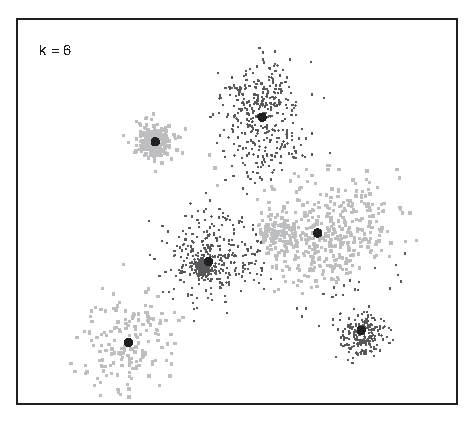
\includegraphics{img/clustershop3}}
  \caption{The result of running the $k$-means algorithm on the data
    from Figure \ref{fig:silhouette1}, finding six clusters.
    Different clusters are shown in black and gray, and the cluster
    centroids are indicated by filled dots.}
  \label{fig:clustershop3}
\end{figure}

Finally, we form the average over all single-point silhouette
coefficients and print the results. Figure \ref{fig:silhouette2} shows
them as a graph.

\begin{figure}
  \centerline{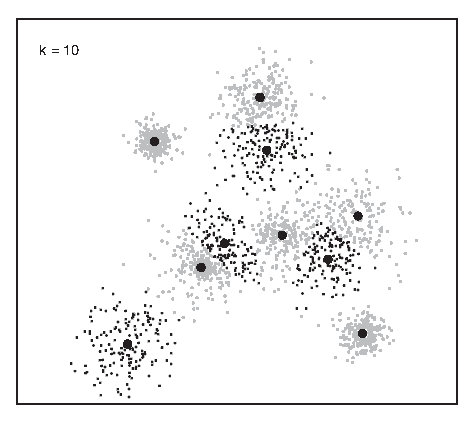
\includegraphics{img/clustershop4}}
  \caption{Similar to Figure \ref{fig:clustershop3} but for $k=10$.
    Ten seems too high a number of clusters for this data set, which
    agrees with the results from calculating the silhouette
    coefficient in Figure \ref{fig:silhouette2}.}
  \label{fig:clustershop4}
\end{figure}

Figures \ref{fig:clustershop3} and \ref{fig:clustershop4} show how the
program assigned points to clusters in two runs, finding 6 and 10
clusters, respectively.\vadjust{\pagebreak}  These results agree with Figure
\ref{fig:silhouette2}: $k=6$ is close~to the optimal number of
clusters, whereas $k=10$ seems to split some clusters artificially.

The next listing demonstrates the \texttt{kmedoids()} function, which
we have to use if we want to provide our own distance function.  As
implemented by the \texttt{Pycluster} library, the $k$-medoids
algorithm does \emph{not} require the data at all---all it needs is
the distance matrix!

\begin{verbatim}
import Pycluster as pc
import numpy as np
import sys

# Our own distance function: maximum norm
def dist( a, b ):
    return max( abs( a - b ) )

# Read data filename and desired number of clusters from command line
filename, n = sys.argv[1], int( sys.argv[2] )

# x and y coordinates, whitespace-separated
data = np.loadtxt( filename, usecols=(0,1) )
k = len(data)

# Calculate the distance matrix
m = np.zeros( k*k )
m.shape = ( k, k )

for i in range( 0, k ):
    for j in range( i, k ):
        d = dist( data[i], data[j] )
\end{verbatim}
\begin{verbatim}
        m[i][j] = d
        m[j][i] = d

# Perform the actual clustering
clustermap = pc.kmedoids( m, n, npass=20 )[0]

# Find the indices of the points used as medoids, and the cluster masses
medoids = \{\}
for i in clustermap:
    medoids[i] = medoids.get(i,0) + 1
\end{verbatim}
\begin{verbatim}

# Print points, grouped by cluster
for i in medoids.keys():
    print "Cluster=", i, " Mass=", medoids[i], " Centroid: ", data[i]

    for j in range( 0, len(data) ):
        if clustermap[j] == i:
            print "\t", data[j]
\end{verbatim}

In the listing, we calculate the distance matrix using the maximum
norm (which is not supplied by \texttt{Pycluster}) as distance
function. Obviously, we could use any other function here---such as
the Levenshtein distance if we wanted to cluster the strings in Figure
\ref{fig:stringscluster}.

We then call the \texttt{kmedoids()} function, \index{kmedoids() function} which returns a
\texttt{clustermap} data structure similar to the one returned by
\texttt{kcluster()}. For the \texttt{kmedoids()} function, the data
structure contains---for each data point---the index of the data point
that is the centroid of the assigned cluster.

Finally, we calculate the masses of the clusters and print the
coordinates of the cluster medoids as well as the coordinates of all
points assigned to that cluster.

The C Clustering Library is small and relatively easy to use.  You
might also want to explore its tree-clustering implementation.  The
library also includes routines for Kohonen maps and principal
component analysis, which we will discuss in Chapter
\ref{ch:reduction}.
  
\index{clustering!Pycluster and the C Clustering Library|)}
\index{Pycluster and the C Clustering Library|)} 
\index{C Clustering Library|)}  

% ============================================================
\section{Further Reading}
\begin{itemize}
\item \cit{Introduction to Data Mining}{Pang-Ning Tan, Michael
    Steinbach, and Vipin Kumar}{Addison-Wesley}{2005}
  This is my favorite book on data mining. The presentation is compact
  and more technical than in most other books on this topic.  The
  section on clustering is particularly strong.

\item \cit{Data Clustering: Theory, Algorithms, and
    Applications}{Guojun Gan, Chaoqun Ma, and Jianhong Wu}{SIAM}{2007}
  This book is a recent survey of results from clustering research.
  The presentation is too terse to be useful, but it provides a good
  source of concepts and keywords for further investigation.

%\item \cit{Introduction to Data Mining}{Pang-Ning Tan et al}{Addison-Wesley}{2005}
%  This is my favorite book on data mining. The presentation is compact
%  and more technical than in most other books on this topic.  The
%  section on clustering is particularly strong.
%
%\item \cit{Data Clustering: Theory, Algorithms, and
%    Applications}{Guojun Gan et al}{SIAM}{2007}
%  This book is a recent survey of results from clustering research.
%  The presentation is too terse to be useful, but it provides a good
%  source of concepts and keywords for further investigation.\vfill\pagebreak

% \item \cit{A Density-Based Algorithm for Disco
%     Spatial Databases with Noise}{Martin Ester, Hans-Peter Kriegel,
%     J\"org Sander, and Xiaowei Xu}{Proceedings of 2nd International
%     Conference on Knowledge Discovery and Data Mining (KDD-96)}{1996}
%   This is the original paper on the DBSCAN algorithm. It can be found
%   on the Web.

\item \cit{Algorithms for Clustering Data}{Anil K.\ Jain and Richard
    C.\ Dubes}{Prentice Hall}{1988}
  An older book on clustering as freely available at
  \url{http://www.cse.msu.edu/}$\sim$\url{jain/Clustering}\_\url{Jain}\_\url{Dubes.pdf}.

\item \cit{Metric Spaces: Iteration and Application}{Victor
    Bryant}{Cambridge University Press}{1985} 
  If you are interested in thinking about distance measures in
  arbitrary spaces in a more abstract way, then this short (100-page)
  book is a wonderful introduction. It requires no more than some
  passing familiarity with real analysis, but it does a remarkable job
  of demonstrating the power of purely abstract reasoning---both from
  a conceptual point of view but also with an eye to real
  applications.
\end{itemize}

\index{data analysis!clustering|)}
\index{clustering|)}

\clearpage

\thispagestyle{empty}

\cleardoublepage